\documentclass[aspectratio=169,11pt]{beamer}
\usetheme{default}
\usefonttheme{professionalfonts}
\usepackage[T1]{fontenc}
\usepackage{lmodern}
\usepackage{amsmath,tikz}
\usetikzlibrary{arrows.meta,positioning}
\definecolor{navy}{RGB}{22,55,92}
\definecolor{blue}{RGB}{44,108,160}
\definecolor{gold}{RGB}{194,137,38}
\definecolor{lightblue}{RGB}{233,241,248}
\definecolor{lightgold}{RGB}{250,243,225}
\definecolor{darkgray}{RGB}{55,62,69}
\setbeamercolor{normal text}{fg=darkgray,bg=white}
\setbeamercolor{frametitle}{fg=navy}
\setbeamercolor{structure}{fg=blue}
\setbeamertemplate{navigation symbols}{}
\setbeamertemplate{frametitle}{\vspace{0.3cm}\insertframetitle\par\vspace{0.08cm}{\color{gold}\rule{\textwidth}{1.2pt}}}
\setbeamertemplate{footline}{\hfill\color{darkgray}\insertframenumber\hspace{0.45cm}\vspace{0.22cm}}

\begin{document}
\begin{frame}{Lineage of irradiation cluster dynamics}
\centering
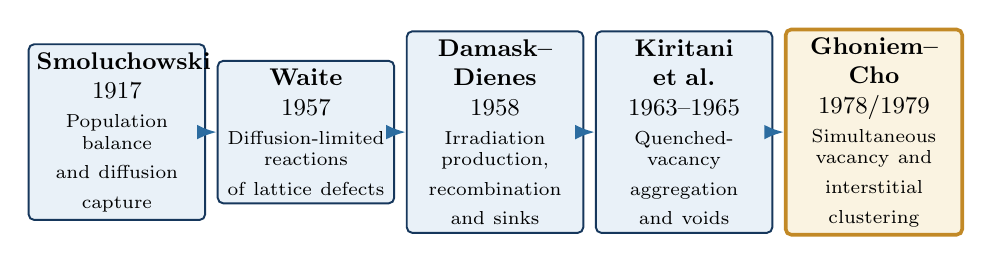
\begin{tikzpicture}[scale=.97,every node/.style={transform shape},
 box/.style={rounded corners=2pt,minimum height=1.25cm,text width=2.10cm,align=center,inner sep=3pt,font=\small,draw=navy,line width=.7pt,fill=lightblue},
 key/.style={box,draw=gold,line width=1.3pt,fill=lightgold},
 arr/.style={-{Latex[length=2.5mm]},line width=1pt,draw=blue}]
\node[box] (s) {\textbf{Smoluchowski}\\1917\\[1mm]\scriptsize Population balance\\and diffusion capture};
\node[box,right=.14cm of s] (w) {\textbf{Waite}\\1957\\[1mm]\scriptsize Diffusion-limited reactions\\of lattice defects};
\node[box,right=.14cm of w] (d) {\textbf{Damask--Dienes}\\1958\\[1mm]\scriptsize Irradiation production,\\recombination and sinks};
\node[box,right=.14cm of d] (k) {\textbf{Kiritani et al.}\\1963--1965\\[1mm]\scriptsize Quenched-vacancy\\aggregation and voids};
\node[key,right=.14cm of k] (g) {\textbf{Ghoniem--Cho}\\1978/1979\\[1mm]\scriptsize Simultaneous vacancy and\\interstitial clustering};
\draw[arr] (s)--(w); \draw[arr] (w)--(d); \draw[arr] (d)--(k); \draw[arr] (k)--(g);
\end{tikzpicture}
\vspace{0.55cm}
\begin{beamercolorbox}[wd=.90\textwidth,sep=.22cm,rounded=true]{block body}
\centering\large\textbf{Key distinction:}\quad the capture kernel appeared first; the coupled evolution of \emph{both} defect-cluster families under continuous irradiation came later.
\end{beamercolorbox}
\vspace{0.35cm}
{\footnotesize $K_{ij}=4\pi(D_i+D_j)R_{ij}$ \hspace{.5cm}$\Longrightarrow$\hspace{.5cm}$\{C_n^v(t),C_n^i(t)\}$ under irradiation}
\end{frame}

\begin{frame}{Position of the Ghoniem--Cho contribution}
\footnotesize
\begin{columns}[T,onlytextwidth]
\begin{column}{.47\textwidth}
\textbf{Before 1978}
\begin{itemize}
\setlength\itemsep{2pt}
\item Smoluchowski population balances
\item Waite $4\pi DR$ defect-reaction coefficients
\item Irradiation production, recombination, and sink loss
\item Vacancy aggregation and void nucleation
\end{itemize}
\end{column}
\begin{column}{.49\textwidth}
\begin{beamercolorbox}[sep=.2cm,rounded=true]{block body}
\textbf{Ghoniem--Cho, 1978/1979}
\begin{itemize}
\setlength\itemsep{2pt}
\item Continuous irradiation source
\item Simultaneous vacancy and interstitial clustering
\item Coupled competition for mobile point defects
\item Influence on early interstitial-loop evolution
\item Time-dependent numerical solution
\end{itemize}
\end{beamercolorbox}
\end{column}
\end{columns}
\vspace{0.08cm}
\begin{block}{Concise priority statement}
An early systematic irradiation cluster-dynamics model---and plausibly the first fully coupled treatment of simultaneous vacancy and interstitial clustering under continuous irradiation.
\end{block}
{\scriptsize\color{darkgray}This does not claim the first Smoluchowski--Waite capture kinetics or the first vacancy-only aggregation model.}
\end{frame}

\begin{frame}{Selected historical references}
\small
\begin{enumerate}
\item M. von Smoluchowski, ``Versuch einer mathematischen Theorie der Koagulationskinetik kolloider L\"osungen,'' \emph{Z. Phys. Chem.} \textbf{92}, 129--168 (1917).
\item T. R. Waite, ``Theoretical Treatment of the Kinetics of Diffusion-Limited Reactions,'' \emph{Phys. Rev.} \textbf{107}, 463--470 (1957). DOI: 10.1103/PhysRev.107.463.
\item G. J. Dienes and A. C. Damask, ``Radiation Enhanced Diffusion in Solids,'' \emph{J. Appl. Phys.} \textbf{29}, 1713--1721 (1958). DOI: 10.1063/1.1723032.
\item J. L. Katz and H. Wiedersich, ``Nucleation of Voids in Materials Supersaturated with Vacancies and Interstitials,'' \emph{J. Chem. Phys.} \textbf{55}, 1414--1425 (1971). DOI: 10.1063/1.1676236.
\item N. M. Ghoniem and D. D. Cho, ``The Influence of Vacancy Clustering on the Early Stages of Interstitial Loop Formation and Growth,'' UCLA-ENG-7845 (August 1978).
\item N. M. Ghoniem and D. D. Cho, ``The Simultaneous Clustering of Point Defects during Irradiation,'' \emph{phys. status solidi (a)} \textbf{54}, 171--178 (1979). DOI: 10.1002/pssa.2210540118.
\end{enumerate}
\end{frame}
\end{document}
